\section{Ejercicio}\label{ej:Chap01Ejercicio03}
Calcular la presión ejercida en el interior del dispositivo cilindro-pistón mostrado en la figura \ref{im:Chap01-001}, el cual contiene aire en su interior, despreciando el peso del gas, si el peso del pistón es $\SI{450}{kg_f}$, su diámetro es de $\SI{300}{mm}$ y sobre este se ejerce la presión atmosférica normal $p_0=\SI{101}{kPa(a)}$. El volumen es de $\SI{500}{l}$ y la temperatura de $\SI{300}{K}$. 

Se pide:
\begin{enumerate}
\item Expresar el resultado de la presión en $\SI{}{kPa(a)}$, $\SI{}{bar(a)}$, $\frac{\SI{}{kg_f}}{\SI{}{cm^2}}\SI{}{(a)}$, $\SI{}{psi(a)}$ y $\SI{}{mca(a)}$.
\item Calcular la presión relativa (manométrica) del aire en el interior del cilindro y expresarla en $\SI{}{kPa(g)}$.
\item Expresar el volumen en $\SI{}{m^3}$ y $\SI{}{ft^3}$.
\item Expresar la temperatura en grados \textit{Celsius} y grados \textit{Fahrenheit}.
\item ¿La presión calculada depende de qué gas se halla en el interior? ¿Y si en el interior hubiera un líquido?
\item Si se calienta el aire, ¿cambia la presión?
\end{enumerate}

\begin{figure}[ht]
\centerline{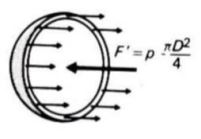
\includegraphics[scale=0.6]{001.jpg}}
\caption{\textit{El dispositivo se encuentra en equilibrio mecánico. El pistón se puede deslizar libremente y sin rozamiento, y no permite fugas.}}
\label{im:Chap01-001}
\end{figure}